In chapter 1, we briefly mentioned the anomaly detection in time series problem and showed that several studies in the literature address different approaches for the problem. 
In chapter 2, we mentioned the models and inference algorithms that are necessary for the development of anomaly detection in time series applications. 
In this chapter, the development of anomaly detection algorithms will be examined. 
Anomaly detection models should be able to distinguish the anomalies arising from the outliers in the system and the anomalies resulting from the errors in the observations.
Besides, these models should be able to cope with missing observations to achieve more fruitful results, because such missing observations may disrupt the resulting anomaly score.
Another issue is the importance of the models that can detect anomalies online because the anomalies are often wanted to be detected as soon as possible, even before they happen.
The rest of this section contains details about the works we have done by paying attention to the above details.

\section{Gaussian Mixture Model for Anomaly Detection}

The problem of anomaly detection is more common in real data than in virtual data. 
Therefore, while modeling the system, it should be ensured that erroneous observations do not disturb the model. 
Therefore, we should be able to model these erroneous observations while developing our model.
In other words, we can say that systems feed on multiple sources where one of them produce erroneous observations.
If we can develop a model in this way, we can better detect system behavior and detect anomalies.
We can develop such a model with Gaussian mixtures.
Let assume; we have a one-dimensional observation. We assume that these observations come from 2 different distributions.
So, we define two distributions. The first one is for non-outlier observations, and it has Gaussian distribution with a mean and ideal amount of variance that is calculated during the expectation maximization process. The second distribution is for outlier observations and has $0$ mean and $\infty$ variance. Then, let us assume, there is another Bernoulli distributed parameter $r$ which decides either given observation is an outlier or not. 
Then, we evaluate the model for parameters of the first distribution during the process. So our generative model is as follows:

\begin{eqnarray}
    r_t &\sim& \mathcal{BE}(\pi) \\
    p\left(y \mid x,r,\mu,\sigma\right) &\sim &\mathcal{N}\left(\mu,\sigma^2\right)^{r=0} \mathcal{N}\left(0,\Sigma\right)^{r=1}
\end{eqnarray}

Here, $r = 1$ represents the outlier observations and $r = 0$ represents the non-outlier ones. 
This model is intended to find the possibility of  $\mu^{(n+1)}$ and $\sigma^{(n+1)}$ which are maximizing the expectation of $\langle \log p\left(y,r\mid x,\mu,\sigma\right)\rangle$ under the probability distribution $p\left(r\mid x,y,\mu^{(n)},\sigma^{(n)}\right)$. So, the derivation of this is as follows:

\begin{eqnarray}
    \mu^{(n+1)},\sigma^{(n+1)}&=&\arg\max_{\mu,\sigma}\mathbb{E}_{p\left(r\mid x,y,\mu^{(n)},\sigma^{(n)}\right)} \left[\log p\left(y,r\mid x,\mu,\sigma\right)\right] \label{eq:mu-sigma}
\end{eqnarray}

If we derive the probability distribution inside the expectation in equation \ref{eq:mu-sigma}, we got the following equations:

\begin{eqnarray}
    p\left(y,r\mid x,\mu,\sigma\right) &=& \prod_t p\left(y_t,r_t\mid x_t,\mu,\sigma\right) \\
    &=&\prod_t p\left(y_t\mid x_t,r_t,\mu,\sigma\right)p\left(r_t\right) \\
    &=&\prod_t \left(\frac{1-\pi_0}{\sqrt{\tau*\sigma^2}}\exp\left(\frac{-(\mu_t-y_t)^2}{2*\sigma_t^2}\right)\right)^{(1-r_t)} \\
    & &\times\left(\frac{\pi_0}{\sqrt{\tau*\Sigma}}\exp\left(\frac{-y_t^2}{2*\Sigma}\right)\right)^{(r_t)} \label{eq:pd}
\end{eqnarray}

After the calculation of $p\left(y,r\mid x,\mu,\sigma\right)$, one can directly calculate the outlier probability $r$ given all other parameters. To calculate $r$, there is a need for the sum of the probability in Equation \ref{eq:pd} over $r$.
The derivation is as follows:

\begin{eqnarray}
    p\left(r\mid x,y,\mu,\sigma\right) &=& \frac{p\left(r,y\mid x,\mu,\sigma\right)}{p\left(y\mid x,\mu,\sigma\right)} \\
    &=& \frac{p\left(r,y\mid x,\mu,\sigma\right)}{\Sigma_r p\left(r,y\mid x,\mu,\sigma \right)}
\end{eqnarray}

From now on, we derived the conditional distribution of outlier probability $r$, $p\left(r\mid x,y,\mu,\sigma\right)$ and opened the formula of $p\left(y,r\mid x,\mu,\sigma\right)$. Now let $\pi_t^{(n)}$ be the probability of $r=1$ given all other parameters. Then $\pi_t^{(n)}$ will become;

\begin{eqnarray}
    \pi_t^{(n)} &=& p\left(r_t=1\mid x_t, y_t, \mu^{(n)} ,\sigma^{(n)}\right) \\
    \pi_t^{(n)} &=& \frac{\frac{\pi_0}{\Sigma}\exp\left(\frac{-y_t^2}{2*\Sigma}\right)}{\frac{\pi_0}{\Sigma}\exp\left(\frac{-y_t^2}{2*\Sigma}\right) + \frac{1-\pi_0}{\sigma}\exp\left(\frac{-(\mu_t-y_t)^2}{2*\sigma^2}\right)}
\end{eqnarray}

Now, we should calculate the log likelihood in the equation \ref{eq:mu-sigma}. The objective is the maximization of the log-likelihood. 
The derivations for the calculation of the log-likelihood is as follows:

\begin{eqnarray}
    \mathbb{E}_{p\left(r\mid x,y,\mu^{(n)},\sigma^{(n)}\right)} \left[\log p\left(y,r\mid x,\mu,\sigma\right)\right] &=&\sum_t \mathbb{E}_{p\left(r\mid x,y,\mu^{(n)},\sigma^{(n)}\right)} \left[\log p\left(y_t,r_t\mid x,\mu,\sigma\right)\right] \nonumber\\
    &=&\sum_t\Bigg\langle r_t\left(\frac{-y_t^2}{2\Sigma^2}\right) \Bigg\rangle \nonumber \\
    &+&\sum_t\Bigg\langle(1-r_t)\left(\left(\frac{-(\mu_t-y_t)^2}{2\sigma_t^2}\right) -log\sigma_t\right)\Bigg\rangle \nonumber\\
    Q(\mu,\sigma)&\propto& \sum_t(1-\pi_t^{(n)})\left(\frac{(\mu_t-y_t)^2}{2\sigma_t^2} + log\sigma_t\right)
\end{eqnarray}

Now, we can iteratively calculate the $\mu^{(n+1)}$ and $\sigma^{(n+1)}$ values that maximize $Q(\mu,\sigma)$ such that;

\begin{eqnarray}
\mu^{(n+1)} &=& \arg\max_{\mu} Q(\mu,\sigma^{(n)}) \\
\sigma^{(n+1)} &=& \arg\max_{\sigma} Q(\mu^{(n)},\sigma)
\end{eqnarray}  

\begin{figure}
    \centering
    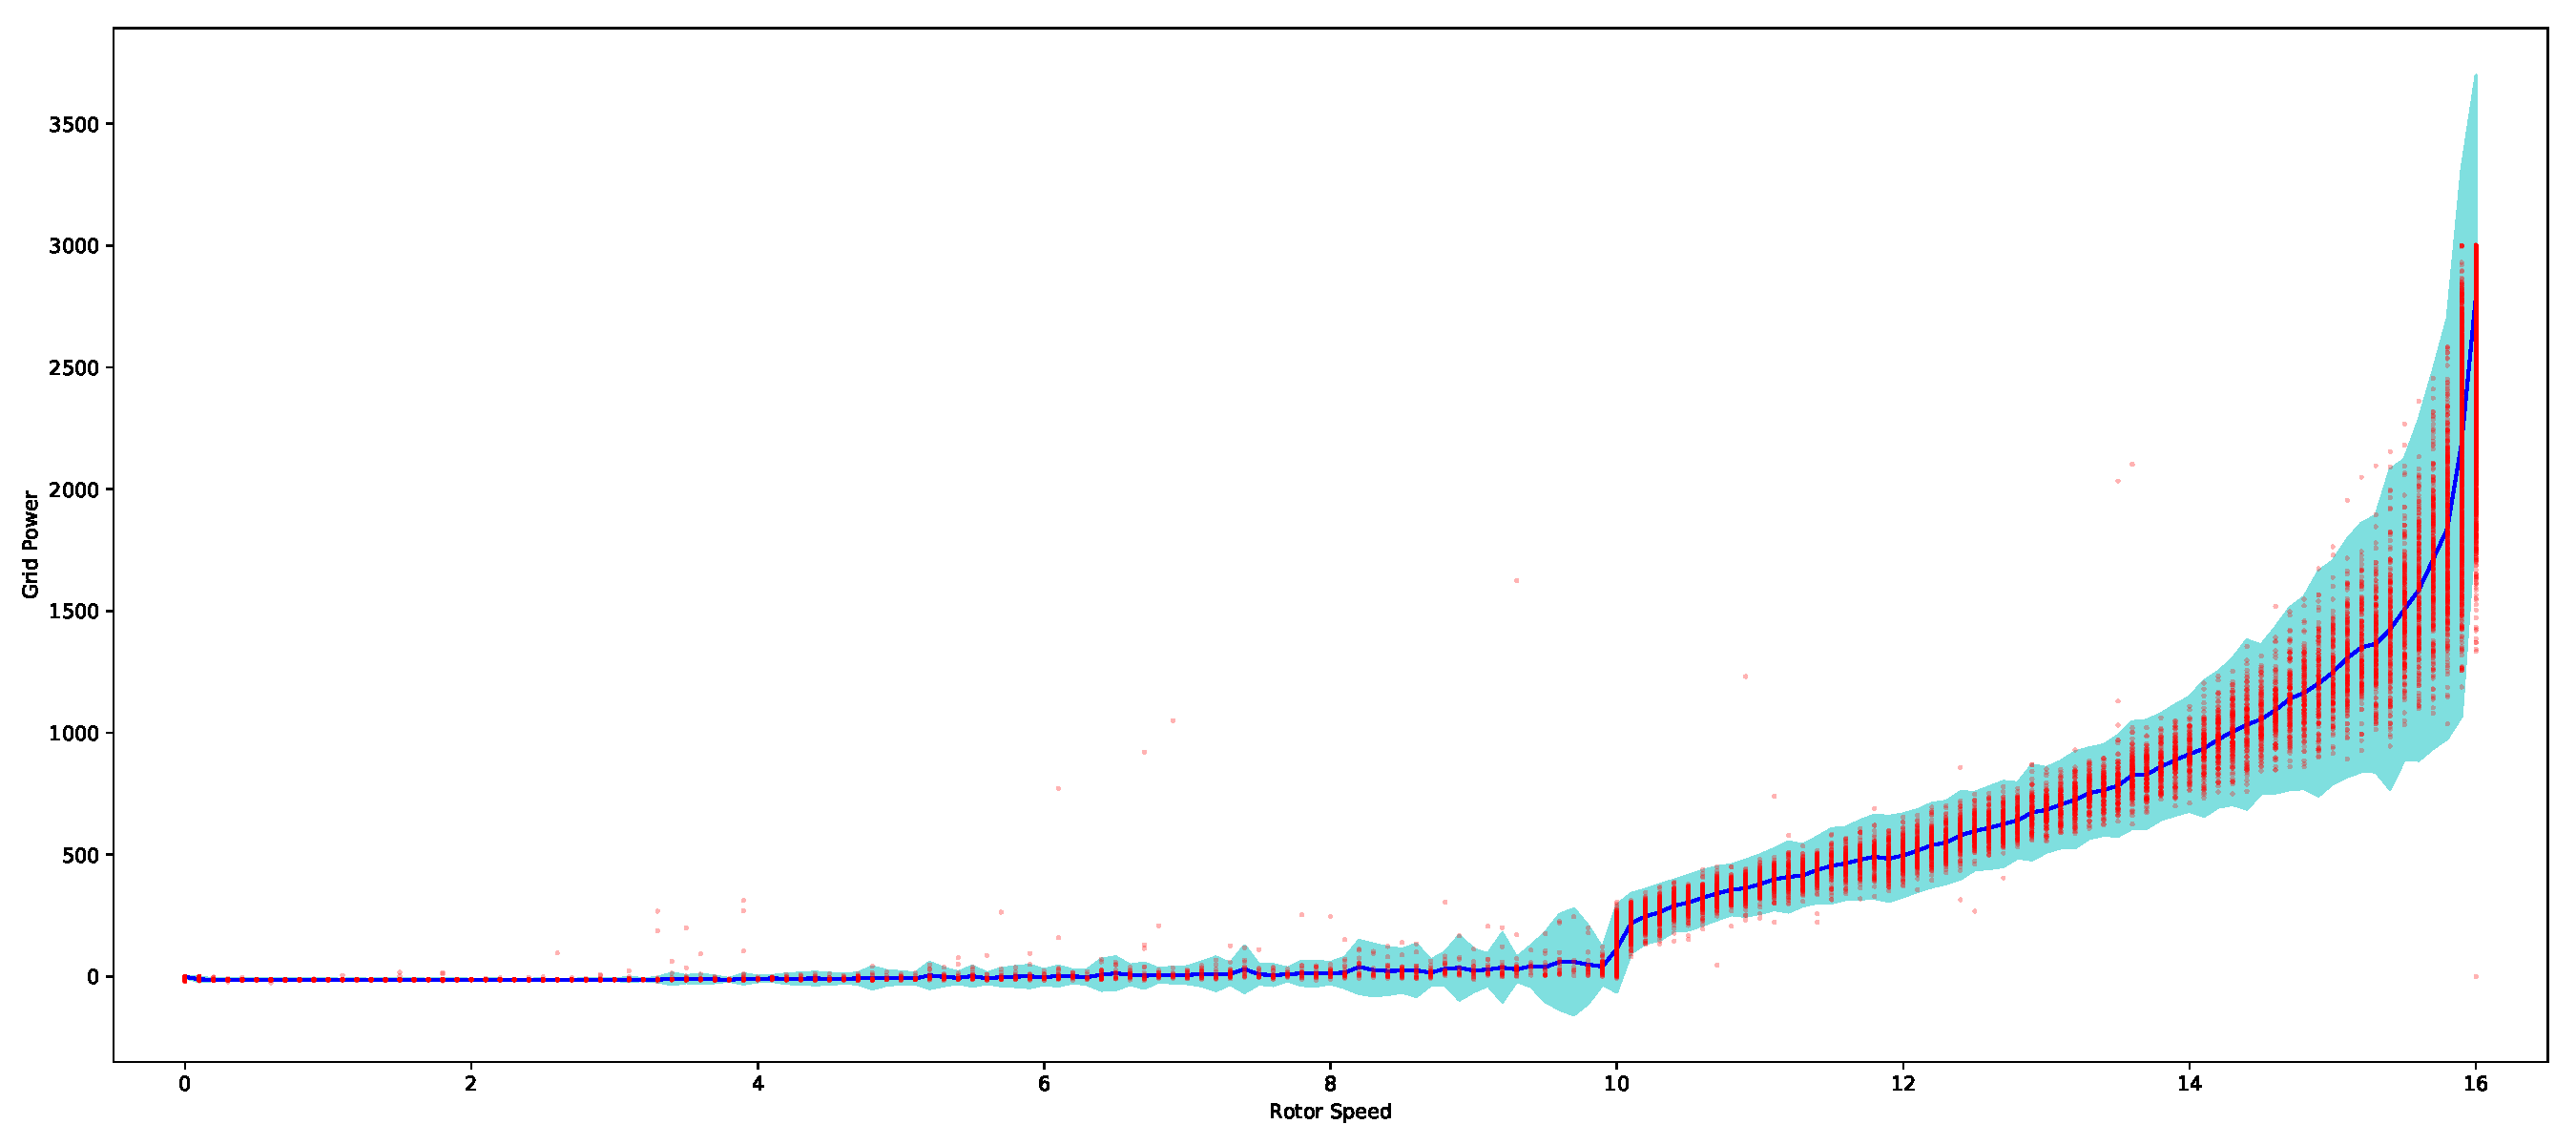
\includegraphics[width=0.85\textwidth]{figures/gmm-em.pdf}
    \caption{One dimensional Gaussian mixtures for the each value on the x-axis}
    \label{fig:gmm-em}
\end{figure}

In this model, we modeled the system without considering time series properties. Figure~\ref{fig:gmm-em} is showing the intuitive but straightforward example of the Gaussian mixtures. The model decides the outlier observations and then learns the system behaviors. The model learns the $r$ parameters during the test, and they will become the anomaly score of the system.

\section{Hidden Markov Model for Anomaly Detection}

The purpose of this section is to create a model that will learn the operation of a system as a time series and generate a warning against distortions and deterioration in this system. 
The model is also expected to catch anomalies in an unsupervised manner because the anomaly detection needs to be done online, and it is often not possible to find the data marked as an anomaly. 
Also, usually, there is not enough data available to model or validate the deterioration phase. 
For this reason, the behavior of the system in normal working conditions has been modeled. The model will generate a warning if the system works outside of the normal working conditions.

In this approach, the behavior of the system is modeled as a \textit{Hidden Markov Model}. 
Also, it is assumed that the system always selects a state from a \textit{discrete state space}, and according to this state, the system creates multi-dimensional observations. 
The state that the system chooses at any time depends only on the previous state. 
This state space corresponds intuitively with the phases that the system enters during operation (such as being closed or working on full power). 
However, one of the main difficulties of the problem is that the data set does not have an attribute, such as the phase of the system. 
Therefore, the state space should be found with the unsupervised learning algorithm. 
There are also some \textit{missing observations} and \textit{outliers} in the data set due to the sensors. 
These are other factors that must be accounted for in the Hidden Markov Model.

In the model, hidden variables of the system for the states at the $t$th time step is shown as $s_t$ and observations of the system at the $t$th time step is shown as $x_t$. 
Observations are usually multi-dimensional and expressed as a vector with a length of $\mathcal{P}+\mathcal{R}$ as $x_t = \begin{bmatrix} p_{t}^{1} & \cdots & p_{t}^{\mathcal{P}} & r_{t}^{1} & \cdots & r_{t}^{\mathcal{R}} \end{bmatrix}^T$. 
There are usually two kinds of the subgroup of observations which are observations that drives the system and observations that are driven by the systems and shown as $p^{1:\mathcal{P}}$ and $r^{1:\mathcal{R}}$, respectively. We will show $p^{1:\mathcal{P}}$ as $p$ and $r^{1:\mathcal{R}}$ as $r$ for the simplicity of the representation, unless otherwise required.

\subsection{Generative Model and Learning}

The discrete state space of the system consists of $S$ different states which indicate the typical operating phases, and there is $1$ additional state which indicates contradictory observations. In fact, with the slight modification of the observation model, instead of defining a separate state for the modeling of contradictory observations, it can be assumed that each observation is observed to be very noisy with a small likelihood. However, as far as we can tell from our analysis, outlier values are more likely to be seen in succession. For this reason, the state space of the model is defined in a way where there is an additional latent feature.

In our model the probability of transitions between states is shown in parameter $\boldsymbol{\Psi} \in \mathbb{R}^{(S+1) \times (S+1)}$. In other words, the transition probability from state $\hat{s}^{\prime}$ to state $\hat{s}$ is $\Psi_{\hat{s}, \hat{s}^{\prime}}$. Each situation has its own observation distribution. The observation distribution where the outliers are observed ($\hat{s}=0$) is a uniform distribution defined in the space of the observation. The observational distributions of the other states ($\hat{s}>0$) are multivariate Gaussian distributions with the variables $\mu_{\hat{s}}$ and $\Sigma_{\hat{s}}$:

\begin{eqnarray}
p(s_1) & = & \mathcal{U}\{0,S\} \\
p(s_{t} =\hat{s} \mid s_{t-1}=\hat{s}^{\prime}) & = & \Psi_{\hat{s} \hat{s}^{\prime}} \\
p(x_{t} \mid s_t = \hat{s}) & = &
\begin{cases}
c,& \hat{s} = 0 \\
\mathcal{N}(x_t;\mu_{\hat{s}},\Sigma_{\hat{s}}),& \hat{s} > 0 \\
\end{cases}
\end{eqnarray}

The next step is to calculate the variables $\Psi_{\hat{s} \hat{s}^{\prime}}$, $\mu_{\hat{s}}$ ve $\Sigma_{\hat{s}}$ from the data. Since this operation is expensive to perform over the whole dataset, random sequences with the length of $ \tau $ can be selected from the dataset. Let $x^{(i)}_{1:\tau}$ be the $i$th selected sequence and suppose that corresponding $s^{(i)}_{1:\tau}$ are known for this sequence. Then sufficient statistics for the variables can be calculated as follows:

{\small
    \begin{eqnarray}
    \Bigl< x_t x_t^T \Bigr>_{p(x_t \mid s_t = \hat{s})} &\approx& \mathcal{V}_{\hat{s}}^{(i)} = \frac{\sum_{t=1}^\tau [s^{(i)}_t = \hat{s}]  x_t x_t^T}{\sum_{t=1}^\tau [s^{(i)}_t = \hat{s}]} \label{eq:suff1}\\
    \Bigl< x_t \Bigr>_{p(x_t \mid s_t = \hat{s})} &\approx& m_{\hat{s}}^{(i)} = \frac{\sum_{t=1}^\tau [s^{(i)}_t = \hat{s}]  x_t }{\sum_{t=1}^\tau [s^{(i)}_t = \hat{s}]}\label{eq:suff2} \\
    C^{(i)}_{\hat{s}\hat{s}^{\prime}} & = & \sum_{t=2}^{\tau} [s^{(i)}_{t-1} = \hat{s}^{\prime}][s^{(i)}_{t} = \hat{s}] \label{eq:suff3}
    \end{eqnarray}
}

The average of sufficient statistics ($\mathcal{V}_{\hat{s}}^{(i)}$, $m_{\hat{s}}^{(i)}$, $C^{(i)}_{\hat{s}\hat{s}^{\prime}}$) of selected sequences can be used to estimate the final values of $\mathcal{V}_{\hat{s}}$, $m_{\hat{s}}$ ve $C_{\hat{s}\hat{s}^{\prime}}$. \textit{Moving averages} can be computed using a $\eta_i$ variable in the range $[0,1]$ to make this process less costly. Estimation of variables of distributions from the sufficient statistics are as follows:

\begin{eqnarray}
\Psi_{\hat{s}\hat{s}^{\prime}} & \approx & C_{\hat{s}\hat{s}^{\prime}}/\sum_k C_{k\hat{s}^{\prime}}  \\
\mu_{\hat{s}} & \approx & m_{\hat{s}}  \\
\Sigma_{\hat{s}} & \approx & \mathcal{V}_{\hat{s}} - m_{\hat{s}} m_{\hat{s}^{\prime}}^T
\end{eqnarray}

The states $s^{(i)}_{1:\tau}$ must be known for the calculations of equations in \ref{eq:suff1}, \ref{eq:suff2} ve \ref{eq:suff3}. If the variables $\Psi_{\hat{s}\hat{s}^{\prime}}$, $\mu_{\hat{s}}$ and $\Sigma_{\hat{s}}$ are known, $s^{(i)}_{1:\tau}$ can be estimated using the following recursive equation with the \textit{Viterbi algorithm}:

\begin{eqnarray}
    \underbrace{\max _{s_{1 : t}^{(i)}} p\left(s_{1 : t}^{(i)}, x_{1 : t}^{(i)}\right)}_{\phi \left(s_{t}^{(i)}\right)}=
    \left(\max _{s_{t}^{(i)}}p\left(x_{t}^{(i)} \mid s_{t}^{(i)}\right) p\left(s_{t}^{(i)} \mid s_{t-1}^{(i)}\right) \right)
    \underbrace{\max _{s_{1 : t-1}^{(i)}} p\left(s_{1 : t-1}^{(i)}, x_{1 : t-1}^{(i)}\right)}_{\phi \left(s_{t-1}^{(i)}\right)}
\end{eqnarray}

Therefore, the desired variables can be deduced by a recursive algorithm which first assumes the states constant and makes \textit{maximization} over the variables and then assumes the variables constant and makes \textit{maximization} over the states.

If there are \textit{missing data}, the only thing that will change is the distribution of observations. Fortunately, one of the advantageous properties of the Gaussian distribution and the uniform distribution is that the \textit{marginal probability} can be easily calculated. For example, in the case where observation $p_*$ is not observed, the distribution with Gaussian joint distribution will be transformed from the $\mu$ and $\Sigma$ into $(\mathcal{P}+\mathcal{R}-1)$ dimensional Gaussian distributions obtained by subtracting all the rows and orders for the observation $p_*$.

\subsection{Calculation of Predictive Distribution}

In the previous section, the process of learning the normal working pattern of the system is performed. After that, the observed behavior should be evaluated with the learned model. In our opinion, calculating the \textit{predictive distribution} to do this task is one of the most efficient ways. One of the important points is that instead of the predictive distribution $p(x_t \mid x_{1:t-1})$ of $x_t$, predictive distribution of the system driven parameters conditioned on the parameter which drives the system $p(r_t \mid p_t, x_{1:t-1})$ is more meaningful. Because the behavior of the system is how the system produces its output under given external conditions.
The predictive distributions of the system driven observations, which are conditional on system driver parameters, are in fact the ratio of the predictive distribution of all observations to the predictive distribution of the system driver observations:

\begin{eqnarray}
p\left(r_t \mid p_t, x_{1:t-1}\right)
& = &  \frac{p\left(x_{t} \mid x_{1:t-1}\right)}{ p\left(p_t \mid x_{1:t-1}\right)}
\end{eqnarray}

Additionally, the predictive distributions of all observations and the predictive distributions of the system driver observations could be calculated by following recursive equations:

\begin{eqnarray}
p\left(x_{t} \mid x_{1:t-1}\right) 
& = & \sum_{s_t} p\left(x_t,s_t \mid x_{1:t-1}\right) \\
& = & \sum_{s_t} p\left(x_t \mid s_t\right) p\left(s_t \mid x_{1:t-1}\right) \\
& = & \sum_{s_t} p\left(x_t \mid s_t\right) \sum_{s_{t-1}} p\left(s_t, s_{t-1} \mid x_{1:t-1}\right) \\
& = & \sum_{s_t} p\left(x_t \mid s_t\right) \sum_{s_{t-1}} p\left(s_t \mid s_{t-1}\right) p\left(s_{t-1} \mid x_{1:t-1}\right) \\
p\left(p_{t} \mid x_{1:t-1}\right) 
& = & \sum_{s_t} p\left(p_t \mid s_t\right) \sum_{s_{t-1}} p\left(s_t \mid s_{t-1}\right) p\left(s_{t-1} \mid x_{1:t-1}\right)
\end{eqnarray}

In order to find $ p \left(s_ {t-1} \mid x_ {1: t-1}\right) $ probabilities in these equations, it is sufficient to find and normalize \textit{forward probabilities}. The forward probabilities can also be found in the following recursive equation:

\begin{eqnarray}
\underbrace{p\left(s_t, x_{1:t}\right)}_{\alpha(s_t)} & = & p\left(x_t \mid s_{t}\right) \sum_{s_{t-1}} p\left(s_t \mid s_{t-1}\right) \underbrace{p\left(s_{t-1}, x_{1:t-1}\right)}_{\alpha\left(s_{t-1}\right)}
\end{eqnarray}

In order to generate anomaly prediction $\mathcal{E}_t$ from predictive distribution, the performance of the predictive distribution calculated by HMM is compared with the performance of the uniform distribution. If the uniform distribution is better than HMM, $\mathcal{E}_t$ will be higher. We foresee these cases as anomalies:

\begin{eqnarray}
\mathcal{E}_t & = & \frac{c}{c+p\left(r_{t} \mid p_t, x_{1:t-1}\right)}
\end{eqnarray}

\section{Deep Learning Sequence Models for Anomaly Detection}

In this section, deep learning models are developed for anomaly detection in time series. 
The developed models in this section are also expected to handle missing observations, and they are developed to find deterioration and anomalies in the system. Since usually there is no deterioration or anomaly label, these model should be an unsupervised model. Therefore, the model uses the system outputs $r$ as a label and trained under system inputs $p$ and system outputs $r$. 
In other words, the model learns the system, not anomalies.
The developed model will perform analysis on time series; therefore, RNNs and LSTMs, which are deep learning sequence models, are used. 
We will decide on the anomalies according to the conformity of the observations to the outputs of the model.

In this approach, we designed deep models that learn the relationship between the system driver parameters (input) and the system driven parameters (output), and the model also learns patterns of the system from the given input. 
Both inputs and outputs are multidimensional and expressed as a vector with the lenghts of $\mathcal{P}$ and $\mathcal{R}$ as $p_t = \begin{bmatrix} p_{t}^{1} & \cdots & p_{t}^{\mathcal{P}} \end{bmatrix}^T$ and $r_t = \begin{bmatrix} r_{t}^{1} & \cdots & r_{t}^{\mathcal{R}} \end{bmatrix}^T$, respectively. 
Therefore the developed models should generate system driven observations from the system driver observations, so it will act as a kind of generative model and learn to generate outputs regarding the system behavior \cite{malhotra2015long}.
Because deep learning sequence models can learn system dynamics in more detail, we prefer to look at the error of the outputs instead of defining an outlier state as in HMM.

\subsection{Forward Propagation in RNN}

The inputs and outputs of the system are defined. Now, in this step, the model is expected to learn the pattern between inputs and outputs. 
Since these networks are expensive to perform over whole dataset, random sequence with length of $\tau$ can be selected at each training epoch. Let $p_{1:\tau}^{(i)}$ be the $i$th selected input sequence and $r_{1:\tau}^{(i)}$ is the corresponding output sequence. The model will calculate the predicted output sequence $\hat{r}_{1:\tau}^{(i)}$.
Forward propagation of RNN for this model is as follows:

\begin{eqnarray}
     s^{\prime}_{t} &=& \mathcal{W}_{ss}s_{t-1} + \mathcal{W}_{sp}p^{(i)}_t + b_s\\ 
     s_{t} &=& h \left(s^{\prime}_{t}\right) \\ 
     \hat{r}^{(i)}_{t} &=& \mathcal{W}_{rs}s_t + c_y \label{eq:rnn-result}
\end{eqnarray}

Where $b_s$ corresponds to bias terms in the hidden layer of the NN and $c_y$ corresponds to bias term in the output layer. $\mathcal{W}$s are the model weights that are learned through training. This forward propagation is calculated from $1:\tau$ for the $i$th subsequence at each epoch. There will be $\mathcal{T}/\tau$ subsequence at each training step. $\mathcal{T}$ corresponds to the number of total data instance.

\subsection{Forward Propagation in LSTM}

In a similar way with the RNN, random sequence with length of $\tau$ can be selected at each training epoch. Let $p_{1:\tau}^{(i)}$ be the $i$th selected input sequence and $r_{1:\tau}^{(i)}$ is the corresponding output sequence. The model will calculate the predicted output sequence $\hat{r}_{1:\tau}^{(i)}$, as in RNN.
The forward propagation of LSTM for such a model is as follows:

\begin{eqnarray}
    f_t & = & \sigma\left(\mathcal{W}^{f}_{ss} s_{t-1} + \mathcal{W}_{sp}^{f} p^{(i)}_t + b^f \right) \\
    \hat{c}_t & = & g\left(\mathcal{W}^{c}_{ss} s_{t-1} + \mathcal{W}_{sp}^{c} p^{(i)}_t + b^c \right) \\
    i_t & = & \sigma\left(\mathcal{W}^{i}_{ss} s_{t-1} + \mathcal{W}_{sp}^{i} p^{(i)}_t + b^i \right) \\
    c_t & = & f_t \odot c_{t-1} + i_t \odot \hat{c}_t \\
    \hat{s}_t & = & h\left(c_{t}\right) \\
    o_t & = & \sigma\left(\mathcal{W}^{o}_{ss} s_{t-1} + \mathcal{W}_{sp}^{o} p^{(i)}_t + b^o \right) \\
    s_t & = & o_t \odot \hat{s}_t \\
    \hat{r}^{(i)}_{t} & = & \mathcal{W}_{rs}s_t + c_y \label{eq:lstm-result}
\end{eqnarray}

Where $b$s correspond to the bias term in the gates and hidden layers, and $c_y$ is the bias at the output layer. $f_t, i_t$ and $o_t$ corresponds to forget gate, input gate, and output gate, respectively. $\hat{c}$ is the proposed cell state, while $c_t$ is the cell state of the network. In a similar manner, $\hat{s}_t$ is the proposed hidden state for the network, while $s_t$ is the filtered and resulted in the hidden state of the network. 

\subsection{Learning}

After the calculation of forward propagation and generation of the $\hat{r}^{(i)}_{1:\tau}$, the loss will be calculated. So, the objective is the minimization of the loss concerning {\boldmath$\mathcal{W}$} which is as follows:

\begin{eqnarray}
    \arg\min_{\boldsymbol{\mathcal{W}}} \mathcal{L} \left(r_{1:\tau}^{(i)} \| \hat{r}_{1:\tau}^{(i)}\right)
\end{eqnarray}

The loss will be calculated and then the weights, $\boldsymbol{\mathcal{W}}$, are updated with the time series specific gradient descent algorithm which is backpropagation through time (BPTT) at each time-step \cite{werbos1990backpropagation}. The forward propagation and the weight update procedure with BPTT algorithm will continue with the new sub-sequences $i^\prime$ at each epoch until the convergence. Thus, the model parameters, $\boldsymbol{\mathcal{W}}$, are learned. As a result of this procedure, the model is able to reproduce system outputs.

\subsection{Prediction and Anomaly Score}

We developed models which learn the system to be analyzed. 
The next step is to find anomalies.
After the training phase, let us assume that there is a sequence, with a length $\mathcal{T}$, and we represent it as $p_{1:\mathcal{T}}$. 
Then the model will calculate the predicted outputs $\hat{r}_{1:\mathcal{T}}$ with the learned weights and bias terms as in the equations \ref{eq:lstm-result} and \ref{eq:rnn-result}.
Then, to detect the anomalies, the loss $\mathcal{L}$ between the observed data $r_{1:\mathcal{T}}$ and model predictions $\hat{r}_{1:\mathcal{T}}$ should be calculated separately for each time step.

\begin{eqnarray}
    \mathcal{E}_t &=& \mathcal{L} \left(r_t \| \hat{r}_t\right)
\end{eqnarray}

We have linear units at the output layer; therefore, our predictions are the result of that linear units.
So, we need to select appropriate loss function. 
{\it Root mean square error} (RMSE), {\it mean square error} (MSE) and {\it mean absolute error} (MAE) are the most appropriate loss functions.
However, since system outputs are multi-dimensional and some of the sensors return numerically large values and dominate the error, such loss functions, especially MSE and RMSE, have drawbacks.
One way to handle this drawback is to use another distance metric, which measures the percentage error. This metric is called as a {\it mean absolute percentage error} (MAPE). However, it brings out other problems such as high error rate at the points where observations are too small.
Therefore, we use another solution.
We normalize all the inputs and outputs and model calculates the results and errors on the normalized data. When doing reconstruction, we unnormalize it. When it comes to producing an anomaly score, we are applying the following steps:

\begin{enumerate}
    \item Calculate the error of each observation and create an unnormalized anomaly score from the error for each observation.
    \item Calculate the average loss of the fake observations which are uniformly selected within the range of the space of the feature space.
    \item Compare unnormalized error with the uniformly selected samples error and create normalized anomaly score.
\end{enumerate}

We compare different loss functions; however, these are not the most appropriate loss functions for our study, except for L1 loss. 
The model we developed performs unsupervised learning. Therefore, our model should not be affected by anomalous observations in the training data while learning the system. 
So, we need a loss function that will not be influenced by the anomalies.
This demand is a severe problem in the robust statistics literature \cite{black1996unification}, and we use the {\it Tukey's biweight} loss function as a robust optimization method for a deep regression \cite{belagiannis2015robust}. 
Detailed analysis of the MSE loss, L1 loss, and Tukey's biweight loss could be found in Appendix \ref{chapter:comparison-of-the-loss-functions}.

Let $c$ represents the average loss of the uniformly selected random samples, and let $\mathcal{E}^{\prime}_t$ shows the unnormalized error for the $t$th observation. Then we can obtain normalized anomaly score with the following equation:

\begin{eqnarray}
\mathcal{E}_t & = & \frac{\mathcal{E}^{\prime}_t}{c+\mathcal{E}^{\prime}_t}
\end{eqnarray}

If there is a higher probability of error for the specified time step, then corresponding observation will be marked as an anomaly. For the detection of collective anomaly \cite{bontemps2016collective}, moving averages of the resulting errors can be computed using a $\eta$ variable in the range $[0,1]$, which is as follows:

\begin{eqnarray}
    \hat{\mathcal{E}}_t &=& \hat{\mathcal{E}}_{t-1} \times \eta + \mathcal{E}_t \times \left(1 - \eta\right)  
\end{eqnarray}

In this section, we developed two similar models which use RNN and LSTM, respectively. It is expected that LSTM should give more precise results if the system has long-term dependencies while RNN should give more accurate results if the system has only short-term dependencies.